% cd /storage/emulated/0/Documents/documents/latex/1920/Grade-10/1st/tangent-lines-and-tangent-circles && pdflatex qz-tangent-lines-and-tangent-circles.tex && termux-open qz-tangent-lines-and-tangent-circles.pdf

% cd /storage/emulated/0/Documents/documents/latex/1819/grade10/visual/4th/tangent-lines-and-tangent-circles && convert -density 600 qz-tangent-lines-and-tangent-circles.pdf -crop 2200x1700 -quality 100 -verbose qz-tangent-lines-and-tangent-circles%02d.png

%2480.5x3508 portrait 2x2 2550x3300
%3508x2480.5 landscape 2x2 3300x2550 
%1653.7x2338.7 portrait 3x3 1700x2200
%landscape 3x3 2200x1700

% cd /storage/emulated/0/Documents/documents/latex/1819/grade10/visual/4th/tangent-lines-and-tangent-circles && while inotifywait -e close_write qz-tangent-lines-and-tangent-circles*.tex; do touch /storage/emulated/0/Android/data/com.termux/files/launch-termux.txt && printf '1' > /storage/emulated/0/Android/data/com.termux/files/launch-termux.txt && pdflatex qz-tangent-lines-and-tangent-circles.tex && termux-open qz-tangent-lines-and-tangent-circles.pdf; done

% cd /host-rootfs/storage/emulated/0/Documents/documents/latex/1819/grade10/visual/4th/tangent-lines-and-tangent-circles && while inotifywait -e close_write qz-tangent-lines-and-tangent-circles*.tex; do pdflatex qz-tangent-lines-and-tangent-circles.tex  && printf "/storage/emulated/0/Documents/documents/latex/1819/grade10/visual/4th/tangent-lines-and-tangent-circles/qz-tangent-lines-and-tangent-circles.pdf" > /host-rootfs/storage/emulated/0/GNURoot/home/Scripts/file-to-launch.txt; done


\documentclass[10pt]{article}
\usepackage[letterpaper, landscape, right=0.25in, left=0.25in, top=0.25in, bottom=0.25in]{geometry}
\usepackage{xcolor}
\usepackage{anyfontsize}
\usepackage{enumitem}
\usepackage{multicol}
\usepackage{amsmath}
%\usepackage{amsfonts,dsfont}% for \mathds 
\usepackage{tabularx} 
\usepackage{gensymb}
\usepackage{multirow}
\usepackage{graphicx, tipa}
\usepackage{tikz}
\usetikzlibrary{angles,quotes}
\usepackage{pgfplots} 
\usetikzlibrary{calc}
\pgfplotsset{compat=newest}
\usetikzlibrary{arrows.meta}
\usetikzlibrary{intersections}
\usetikzlibrary{decorations.pathreplacing}
\usepackage{flafter}
\usepackage{amsmath,amssymb,cancel,units}
\usepackage{microtype} % nicer output 
\usepackage{hfoldsty} % nicer output 
\usepackage{fixltx2e} 
\usepackage{mathptmx}
%\usepackage{booktabs}
\usepackage{numprint}
\usepackage[utf8]{inputenc} 
\usepackage[T1]{fontenc}
%\usepackage{siunitx} 
%\sisetup{detect-all}


\def\radA{3.6cm}

\def\radB{3.6cm}

%\def\thirdrad{8cm}

\pagenumbering{gobble}
%\linespread{0.9}
\newcommand{\vspce}{\vspace{0.75ex}}
\newcommand{\hspce}{\hspace{0.5em}}
\newcommand{\blank}{\underline{\hspace{2em}}}%{\rule{1em}{0.15ex}}
\newcommand{\arc}[1]{{% 
\setbox9=\hbox{#1}% 
\ooalign{\resizebox{\wd9}{\height}{\texttoptiebar{\phantom{A}}}\cr#1}}}

\newcolumntype{C}{ >{\centering\arraybackslash} X}




\begin{document}
\boldmath
{\fontsize{38}{40}\fontfamily{pnc}\selectfont {

\input{qz-tangent-lines-and-tangent-circles-input}

%}} 

%\newpage

%{\fontsize{30}{35}\fontfamily{pnc}\selectfont {

%\def\currentdir{/storage/emulated/0/Documents/documents/latex/1920/Grade-10/2nd/tangent-lines-and-tangent-circles}

\vspace*{0.3cm}
\begin{center}
\scalebox{1}{
\noindent\begin{minipage}{\textwidth}

{\begin{multicols}{2}
3. \hspace*{1.5cm}
\begin{tikzpicture}[
remember picture, overlay, 
baseline = (current bounding box.west)
]  

\def\radE{0.5cm}

\def\radF{0.7cm}

\coordinate (intE) at (0,0); 

\coordinate (intF) at (1.5*\radF,0); 

\node(e) at ($(intE)+(90:\radE)$) {};

\draw[line width=0.5mm] (e) node[circle, fill=black, inner sep=0pt, outer sep=0pt, minimum size=3pt] {} circle [radius=\radE];

\node(e-label) at ($(e)+(50:0.3*\radF)$) {$  E$};

\draw[line width=0.3mm, <->, >={Latex[round]}] ($(intE) +(180:1.2*\radE)$) -- ($(intF) +(0:1.2*\radF)$);

\node(f) at ($(intF)+(-90:\radF)$) {};

\node(n) at ($(intF)+(15:1cm)$) {$  n$};

\draw[line width=0.5mm] (f) node[circle, fill=black, inner sep=0pt, outer sep=0pt, minimum size=3pt] {} circle [radius=\radF];

\node(f-label) at ($(f)+(-50:0.3*\radF)$) {$  F$};

\end{tikzpicture}

 %& 
4. \hspace*{1.5cm}\begin{tikzpicture}[remember picture, overlay, 
baseline = (current bounding box.north)
]  
 
\pgfmathsetmacro{\rone}{1} 

\pgfmathsetmacro{\rtwo}{0.6}
 
\pgfmathsetmacro{\mid}{\rone/(\rone + \rtwo)} 

\pgfmathsetmacro{\out}{\rone/(\rone - \rtwo)} 

\node[draw,circle,minimum size=2 * \rone cm,inner sep=0pt, line width=0.5mm] (c1) at (2*\rone,0) {}; 

\node[draw,circle,minimum size=2 * \rtwo cm,inner sep=0pt, line width=0.5mm] (c2) at (0,0) {}; 

\path (c1.center) -- node[coordinate,pos=\mid] (mid) {} (c2.center); 

\path (c1.center) -- node[coordinate,pos=\out] (out) {} (c2.center); 

\draw(c1.center) node  [circle, fill=black, inner sep=0pt, outer sep=0pt, minimum size=3pt] () {};

\draw(c2.center) node  [circle, fill=black, inner sep=0pt, outer sep=0pt, minimum size=3pt] () {};

\node(i-label) at ($(c1.center)+(180:0.22*\rone)$) {$  I$};

\node(h-label) at ($(c2.center)+(180:0.22*\rone)$) {$  H$};

\foreach \i in {1,2} 
\foreach \j in {1,2} 
\foreach \k in {mid,out} 
\coordinate (t\i\j\k) at (tangent cs:node=c\i,point={(\k)},solution=\j); 

\foreach \i in {1,2} 
\foreach \k in {mid,out} 
\draw[line width=0.3mm, <->, >={Latex[round]}] ($(t1\i\k)!-1cm!(t2\i\k)$) -- ($(t2\i\k)!-0.8cm!(t1\i\k)$); 

\node(p-label) at ($(t21mid)!-1cm!(t11mid)+(110:3pt) $) {$  p$};

\node(s-label) at ($(t22mid)!-1cm!(t12mid)+(-110:3pt) $) {$  s$};

\node(r-label) at ($(t21out)!-1cm!(t11out)+(-70:0.25*\rone) $) {$  r$};

\node(q-label) at ($(t22out)!-1cm!(t12out)+(70:0.25*\rone) $) {$  q$};

\end{tikzpicture}

 %\\
\end{multicols}}
\end{minipage}}
\end{center}   

\vspace*{1.3cm}
B. In $\odot{O}$, $\overline{CT}$, $\overline{ET}$ are tangent segments and $m$ is tangent to $\odot{O}$ at S. 
\begin{center}
\vspace*{-2ex}
\scalebox{1}{
\noindent\begin{minipage}{\textwidth}
{
\begin{enumerate}[label = \arabic*. ]
\item $m\angle{OCT}=$ \blank. 
\item $m\angle{OSI}=$ \blank. %\hspace*{8cm}\begin{tikzpicture}[remember picture, overlay
]

\def\rad{1.2cm}

\node[draw,circle,minimum size=2*\rad,inner sep=0pt, line width=0.5mm, outer sep=0] (c1) at (0,0) {}; 

\node(o-label) at ($(c1.center)+(150:0.22*\rad)$) {$  O$};

\coordinate (t) at (0,-3*\rad); 

\node(t-label) at ($(t)+(270:0.22*\rad)$) {$  T$};

\draw[line width=0.3mm] (c1.center) -- (tangent cs:node=c1, point={(t)}, solution=1) -- (t) -- (tangent cs:node=c1, point={(t)}, solution=2) -- cycle; 

\node(e-label) at ($(tangent cs:node=c1, point={(t)}, solution=1)+(-20:0.2*\rad)$) {$  E$};

\node(c-label) at ($(tangent cs:node=c1, point={(t)}, solution=2)+(200:0.2*\rad)$) {$  C$};

\coordinate (n) at (90:\rad); 

\node(n-label) at ($(n)+(90:0.2*\rad)$) {$  N$};

\coordinate (s) at (-90:\rad); 

\node(s-label) at ($(s)+(-90:0.2*\rad)$) {$  S$};

\node[circle, fill=black, inner sep=0pt, outer sep=0pt, minimum size=3pt] (i) at ($(s)+(180:\rad)$) {};

\coordinate (l) at ($(s)+(180:1.2*\rad)$); 

\node(i-label) at ($(i)+(90:0.2*\rad)$) {$  I$};

\coordinate (m) at ($(s)+(0:1.2*\rad)$); 

\node(l-label) at ($(m)+(90:0.2*\rad)$) {$m$};

\draw[line width=0.3mm] (n) -- (s); 

\draw[line width=0.3mm, <->, >={Latex[round]}] (l) -- (m); 

\end{tikzpicture}
 \vspace*{-2.5ex}
\item If $\overline{SN}=24$ units,  then $\overline{OE}=$ \blank. 
\item If $\overline{OS}=5$ units and $\overline{SI}=12$ units,\newline then $\overline{OI}=$ \blank. 
\item If $\overline{CT}=15$ units,  then $\overline{ET}=$ \blank. 
\item If $\overline{OC}=8$ units and\newline $\overline{ET}=15$ units,  then $\overline{OT}=$ \blank. 
\item If $\overline{OE}=11$ units, then $\overline{NS}=$ \blank. 
\item If $\overline{OS}=7$ units and  $\overline{OT}=25$ units,\newline then $\overline{CT}=$ \blank. 
\end{enumerate}  

\vspace*{-5cm}\hspace*{8.5cm}\begin{tikzpicture}[remember picture, overlay
]

\def\rad{1.2cm}

\node[draw,circle,minimum size=2*\rad,inner sep=0pt, line width=0.5mm, outer sep=0] (c1) at (0,0) {}; 

\node(o-label) at ($(c1.center)+(150:0.22*\rad)$) {$  O$};

\coordinate (t) at (0,-3*\rad); 

\node(t-label) at ($(t)+(270:0.22*\rad)$) {$  T$};

\draw[line width=0.3mm] (c1.center) -- (tangent cs:node=c1, point={(t)}, solution=1) -- (t) -- (tangent cs:node=c1, point={(t)}, solution=2) -- cycle; 

\node(e-label) at ($(tangent cs:node=c1, point={(t)}, solution=1)+(-20:0.2*\rad)$) {$  E$};

\node(c-label) at ($(tangent cs:node=c1, point={(t)}, solution=2)+(200:0.2*\rad)$) {$  C$};

\coordinate (n) at (90:\rad); 

\node(n-label) at ($(n)+(90:0.2*\rad)$) {$  N$};

\coordinate (s) at (-90:\rad); 

\node(s-label) at ($(s)+(-90:0.2*\rad)$) {$  S$};

\node[circle, fill=black, inner sep=0pt, outer sep=0pt, minimum size=3pt] (i) at ($(s)+(180:\rad)$) {};

\coordinate (l) at ($(s)+(180:1.2*\rad)$); 

\node(i-label) at ($(i)+(90:0.2*\rad)$) {$  I$};

\coordinate (m) at ($(s)+(0:1.2*\rad)$); 

\node(l-label) at ($(m)+(90:0.2*\rad)$) {$m$};

\draw[line width=0.3mm] (n) -- (s); 

\draw[line width=0.3mm, <->, >={Latex[round]}] (l) -- (m); 

\end{tikzpicture}
 \vspace*{5cm}
}
\end{minipage}}
\end{center}  



}}


\end{document}